% !TeX program = xelatex
% Multimodal CSL Recognition — English restructured report
% Built following the Light-Skills IMRaD template (skills/light-paper-writing/templates/01_imrad.md)
\documentclass[11pt,a4paper]{article}

\usepackage[margin=2.4cm]{geometry}
\usepackage{graphicx}
\usepackage{booktabs}
\usepackage{amsmath,amssymb}
\usepackage{array}
\usepackage{multirow}
\usepackage{caption}
\usepackage{float}
\usepackage{enumitem}
\usepackage{xcolor}
\usepackage[hidelinks]{hyperref}
\usepackage{titlesec}
\usepackage{authblk}

\graphicspath{{figs_en/}}
\captionsetup{font=small,labelfont=bf,skip=6pt}
\setlength{\parskip}{3pt}
\titleformat{\section}{\normalfont\large\bfseries}{\thesection}{0.7em}{}
\titleformat{\subsection}{\normalfont\normalsize\bfseries}{\thesubsection}{0.6em}{}

\title{\bfseries Multimodal Chinese Sign Language Recognition\\[2pt]
with Strain/Pressure and sEMG Sensing\\[10pt]
\normalfont\normalsize Reproduction of a Reported Fusion Gain\\[1pt]
and Evidence of Dominant-Modality Degeneration}
\author{}
\date{October 2026}

\begin{document}
\maketitle

\begin{abstract}
\noindent
A common premise in wearable sign-language recognition is that adding surface electromyography (sEMG) to strain/pressure sensing improves recognition accuracy relative to either modality alone; the reference system we study reports a $+15.9$\,pp gain from doing so. We reproduce a recently reported ion-conductive hydrogel system on its 24-class Chinese Sign Language dataset (2{,}880 samples; 8:1:1 file-level split) and verify the split is byte-identical across two environments. Our from-scratch dual-branch Bi-LSTM reaches 98.61\% single-run test accuracy and $98.96\pm0.40$\% across four random seeds, matching the source paper's fusion result (99.65\%) within seed variance; a TCN comparator reaches $99.42\pm0.40$\%. However, three independent experiments show the fusion is nominal. Inference pruning leaves \emph{every one of the 288 test predictions unchanged} when sEMG is zeroed (288/288 identical), whereas zeroing the glove input collapses accuracy to chance (4.17\%); modality dropout during training fails to change this behaviour, with training accuracy pinned at 0.7617; and an oracle upper bound equals the observed score in four of five configurations, leaving 0.00\,pp of theoretically reachable improvement. We further falsify an intuitive remedy: band-pass filtering sEMG to remove drift and power-line interference \emph{reduces} single-modality accuracy by 13.55\,pp, indicating the low-frequency content is discriminative. We attribute the divergence from the source paper to a dominant-modality regime: when one modality already separates nearly all samples, gradient descent does not learn the second branch.
\end{abstract}

\noindent\textbf{Keywords:} sign language recognition; surface electromyography; strain/pressure sensing; multimodal fusion; dominant modality; reproducibility

%=====================================================================
\section{Introduction}

Wearable sensing is a practical route to automatic sign-language recognition: strain and pressure sensors embedded in a glove capture finger flexion and palm contact, while surface electromyography (sEMG) captured at the forearm reflects the underlying muscle activation. Because the two signals originate from different physical processes --- one mechanical, one electrophysiological --- multimodal fusion is commonly expected to add accuracy over either channel alone, and recent work reports large gains from doing so.

The specific system we study reports a 24-class Chinese Sign Language task in which fusion reaches 99.65\% accuracy, while strain/pressure alone drops to 83.75\% and sEMG alone to 88.02\% --- an apparent $+15.9$\,pp benefit from fusion. That figure carries a strong implicit claim: that the second modality supplies information the first cannot. If true, it makes multimodal wearable sensing compelling; if the gain instead reflects a specific evaluation protocol or a dataset in which one channel is unusually easy, the conclusion does not generalise.

Reproducing such a claim requires more than re-running an architecture. Three things must hold: the data split must be identical, the preprocessing must not leak evaluation information, and the reported number must be distinguishable from random-seed variation. In our setting the dataset is small (2{,}880 samples, 288 held out for testing), so a difference of two test samples moves accuracy by 0.7\,pp --- comparable to the whole claimed fusion benefit once other factors are accounted for. This motivates an evaluation whose resolution is adequate to the claim.

We therefore build the full pipeline from scratch --- data audit, leakage-checked preprocessing, a fixed stratified split, dual-branch Bi-LSTM fusion aligned to the reference architecture, and four groups of controlled experiments --- and we augment it with analyses that test \emph{mechanism} rather than only accuracy. Specifically, we ask which branch the trained fusion model actually uses at inference; whether training-time interventions can force both branches to contribute; how much improvement is theoretically reachable; and whether the intuitive signal-processing remedy (filtering drift and power-line interference out of sEMG) helps.

Our results are as follows. First, the pipeline reproduces the reference accuracy: 98.61\% single-run and $98.96\pm0.40$\% over four seeds, with TCN comparators at $99.42\pm0.40$\%. Second, and unexpectedly, the fusion model is \textbf{functionally unimodal}: zeroing the sEMG input changes no prediction at all (288/288 identical), while zeroing the glove input reduces accuracy to chance. Modality dropout fails to alter this, and an oracle bound shows that no fusion strategy can exceed the current score in four of five configurations. Third, we falsify a common preprocessing assumption: band-pass filtering sEMG removes 43\,pp of its low-frequency energy but costs 13.55\,pp of single-modality accuracy, so that energy is informative rather than noise. Together these findings indicate a \emph{dominant-modality} regime in which the glove channel alone already separates nearly every sample, leaving no gradient signal for the second branch.

\noindent\textbf{Contributions.}
\begin{itemize}[leftmargin=1.4em,itemsep=1pt]
\item \textbf{C1.} We provide a leakage-audited, seed-controlled reproduction of the reference multimodal sign-language system on its own dataset, including a byte-identical split verification across two environments, and we match the reported fusion accuracy within seed variance.
\item \textbf{C2.} We demonstrate with three mutually independent experiments --- inference pruning, modality dropout, and an oracle upper bound --- that the fused model is functionally unimodal and that its sEMG branch contributes exactly zero to the decision.
\item \textbf{C3.} We quantify four effects usually left implicit: seed variance (0.40\,pp), near-duplicate inflation ($+0.52$\,pp), cross-GPU trajectory divergence at fixed seed, and we falsify the low-frequency-noise filtering hypothesis ($-13.55$\,pp).
\end{itemize}

%=====================================================================
\section{Related Work and Background}

\textbf{sEMG-based gesture and sign recognition.} sEMG from forearm electrodes is a standard input for hand-gesture classification; typical pipelines band-pass the signal, extract time-domain or spectral features, and classify with recurrent or convolutional networks. Reported accuracy depends strongly on the number of classes and on whether electrodes are re-donned between sessions. Our dataset contains a strong narrow-band interference component near 48\,Hz plus low-frequency drift, a condition often handled by notch and high-pass filtering --- a remedy we test directly in Section~\ref{sec:mech}.

\textbf{Strain and pressure sensing for hand pose.} Resistive and capacitive sensors embedded in gloves measure finger flexion and contact pressure. Because they capture the mechanical configuration of the hand rather than the muscle activity that produces it, they are comparatively robust to electrode placement. In our dataset this channel alone reaches 98--99\% accuracy, which turns out to be decisive for the interpretation of the fusion result.

\textbf{Multimodal fusion and modality imbalance.} Multimodal architectures typically encode each modality with a separate branch and fuse by concatenation, summation or attention. A recurring failure mode is \emph{modality imbalance} or \emph{dominant modality}: when one branch converges faster or its modality is intrinsically easier, the classifier learns to rely on it and the other branch receives vanishingly small gradients, effectively dropping out of the computation. Standard remedies include gradient balancing (GradNorm, PCGrad), modality dropout, and auxiliary per-branch supervision. Our contribution here is not a new remedy but evidence that, on this dataset, the ceiling itself is zero --- which makes such remedies unproductive regardless of implementation quality.

\textbf{Reference system.} The system we reproduce reports a dual-branch Bi-LSTM fusion with asymmetric branch widths (128 units for the glove branch, 512 for sEMG), trained with AdamW, batch size 50, learning rate $10^{-3}$ and dropout 0.3 on an 8:1:1 split. It reports 99.65\% fused, 83.75\% glove-only and 88.02\% sEMG-only.

%=====================================================================
\section{Methods}
\label{sec:methods}

\subsection{Dataset}

The dataset contains 24 classes of Chinese Sign Language, each performed 120 times, giving 2{,}880 samples stored as individual \texttt{.pkl} files. Each file is a dictionary with four fixed keys (Table~\ref{tab:data}). Strain/pressure channels are sampled at 200\,Hz and sEMG at 1000\,Hz, so the two modalities have different sequence lengths (400 and 1950) and are encoded by separate branches rather than being time-aligned. A full scan of all 2{,}880 files found no missing keys, NaNs, or Inf values.

The dataset comes from a coursework recording and is not publicly redistributable. It contains no personally identifying information, and we recruited no new human participants for this study. We make the fixed split assignment, per-run summaries, per-sample test predictions and the scripts that reproduce every table in this report available on request. Sign-language glosses appear as classification labels only.

\begin{table}[htbp]\centering
\caption{Dataset structure. Channel counts differ between modalities, so no time alignment is imposed.}
\label{tab:data}
\begin{tabular}{llccc}
\toprule
Key & Modality & Shape & Sampling rate & Duration \\
\midrule
\texttt{res1}, \texttt{res2} & left / right strain--pressure & $(20,400)$ & 200\,Hz & 2.0\,s \\
\texttt{muscle1}, \texttt{muscle2} & left / right sEMG & $(10,1950)$ & 1000\,Hz & 1.95\,s \\
\bottomrule
\end{tabular}
\end{table}

\subsection{Data audit and preprocessing}

Two data properties required treatment. First, strain/pressure contains extreme outliers: the maximum magnitude in \texttt{res2} reaches 3{,}988 whereas typical samples are of single-digit magnitude; the affected files cluster in a few classes. Second, eight of the forty concatenated glove channels carry no dynamic information: their within-sample standard deviation is $0.006$ and their global standard deviation $0.016$, against $0.3$--$93$ for informative channels. Left untreated, these channels would be amplified into spurious features by per-channel standardisation.

The preprocessing order is therefore: (i) clip each channel at the 1st/99th percentile of the \emph{training} split; (ii) standardise per channel using the mean and standard deviation computed \emph{after} clipping and \emph{only} on the training split; (iii) zero the eight noise-floor channels. All statistics are computed once from the training split and then applied unchanged to validation and test. Reversing steps (i) and (ii) leaves the normalised standard deviation at 0.756 instead of 1.0, confirming the order matters.

\subsection{Split protocol and leakage audit}

We stratify the split by class at file level, 8:1:1, giving 2{,}304 / 288 / 288 samples; every class contributes exactly 96 / 12 / 12. We fix the seed and write the assignment to a metadata file that all experiments read, so no run recomputes it. We verified that the three index sets are pairwise disjoint, their union is exactly 2{,}880, and that the metadata labels agree with the data arrays. Normalisation statistics derive only from the training split, and we evaluate the test split once, after training. We compare the split file hash across environments to confirm that both machines used identical members (Section~\ref{sec:env}).

One further property is measured rather than assumed: because the same gesture is repeated 120 times, some repetitions are near-identical. In the glove modality, 79 of 288 test samples (27.4\%) have a training-set neighbour with cosine similarity $\geq 0.999$, all of them same-class. Stratifying test accuracy by this criterion gives 100.00\% on the near-duplicate subset versus 98.09\% on the remainder, i.e. the effect inflates overall accuracy by $+0.52$\,pp (fusion) and $+1.82$\,pp (sEMG-only). This is a property of repeated-trial data under a random split, not a leak in the splitting code, and we report it rather than removing it, because the reference protocol is a random 8:1:1 split.

\subsection{Model architecture}

The model is a dual-branch Bi-LSTM with late feature fusion, aligned with the reference architecture (Figure~\ref{fig:arch}). The glove branch consumes $(B,400,40)$ and applies three stacked bidirectional LSTM layers with hidden size 128, followed by two fully connected layers (256, 128). The sEMG branch consumes $(B,1950,20)$ with three stacked Bi-LSTM layers of hidden size 512 and the same two-layer head. The two 128-dimensional outputs are concatenated and passed through dropout (0.3) and a linear classifier over 24 classes. The asymmetric branch widths follow the reference design. Total parameter count is 16.15\,M.

For the comparison study we additionally implement 1D-CNN, Bi-GRU, TCN and Transformer variants behind the same interface, so that all models receive identical inputs and training budgets.

\begin{figure}[htbp]\centering
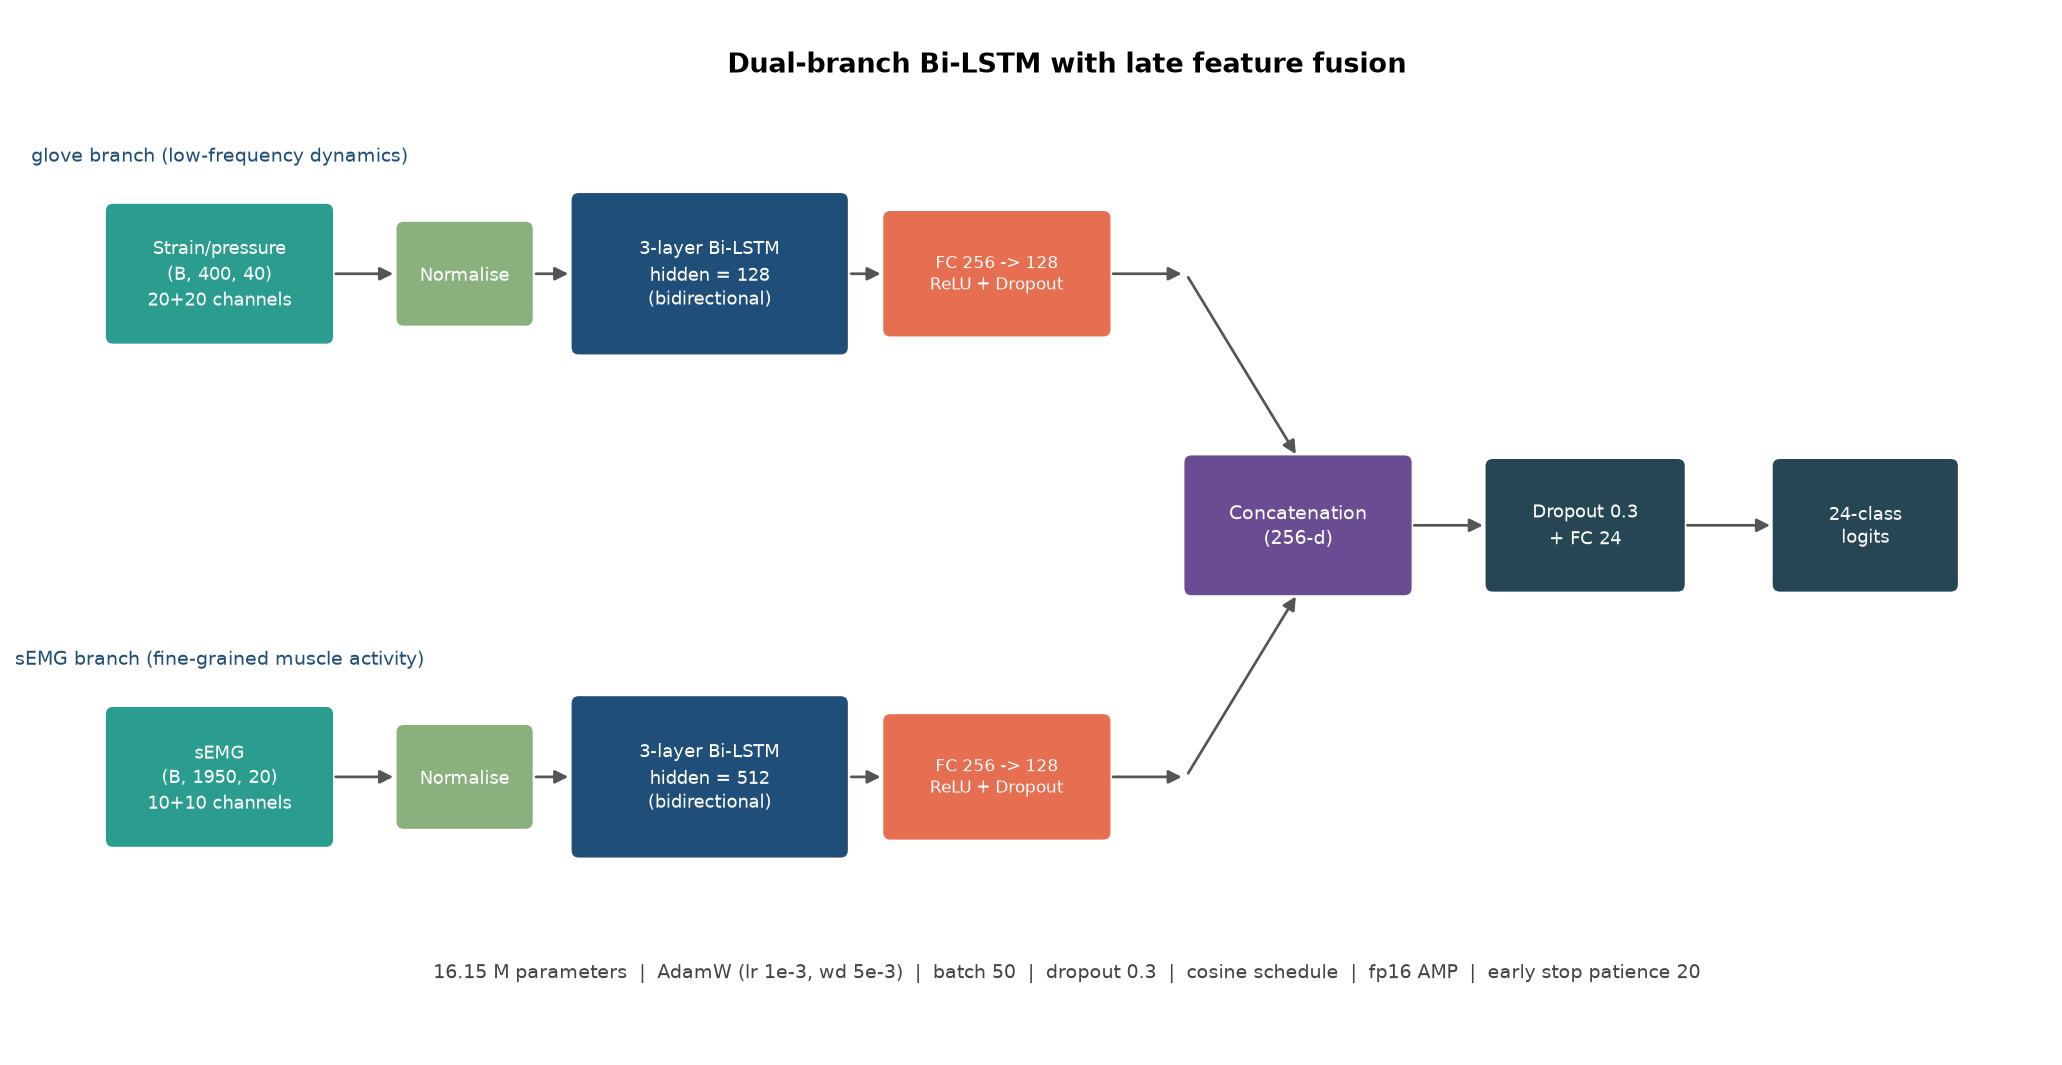
\includegraphics[width=\textwidth]{fig1_architecture.png}
\caption{Dual-branch Bi-LSTM fusion architecture. The glove branch encodes low-frequency mechanical dynamics with 128 hidden units; the sEMG branch encodes fine-grained muscle activity with 512. Branch outputs are concatenated before classification.}
\label{fig:arch}
\end{figure}

\subsection{Training protocol}

All models use AdamW ($\beta$ defaults, weight decay $5\times10^{-3}$) with cosine-annealed learning rate, gradient-norm clipping at 5.0, and early stopping with patience 20 epochs. The reference configuration is batch size 50, learning rate $10^{-3}$ and dropout 0.3. Because the dual-branch model requires 10.66\,GB at batch 50 in full precision, exceeding the 8\,GB of environment A, we enable fp16 automatic mixed precision, which reduces the peak to 5.46\,GB and allows the reference batch size to be reproduced exactly rather than approximated.

\subsection{Experimental environment and cross-environment consistency}
\label{sec:env}

Experiments were run on two environments sharing identical code, data, seed and library versions (Python 3.13, PyTorch 2.9.1+cu126). Environment A has an RTX 4070 Laptop GPU (8\,GB) and environment B an RTX 4080 SUPER (32\,GB). The data split file produced independently on each environment is byte-identical (MD5 \texttt{51c86320\ldots}, 81{,}627 bytes), which establishes that train/validation/test membership is the same.

Running the same configuration (dual-branch Bi-LSTM, seed 42, 100-epoch budget) on both environments gives 98.61\% (environment A) and 99.31\% (environment B). The training trajectories diverge from the first epoch (21.88\% vs 18.06\% validation accuracy) because cuDNN selects different convolution algorithms depending on the GPU, changing floating-point accumulation order. The 0.70\,pp gap corresponds to two test samples and lies inside the $\pm1.2$\,pp confidence interval of a 288-sample test set. We therefore perform all horizontal comparisons \emph{within} one environment and do not compare absolute values across environments; conclusions that depend on randomness use the multi-seed statistics of Section~\ref{sec:main}.

%=====================================================================
\section{Experiments and Results}
\label{sec:results}

\subsection{Setup and metrics}

Unless stated otherwise, experiments use the fixed split, the reference hyperparameters, and are evaluated once on the 288-sample test set. Model selection uses the validation split only. Because a single test set of this size resolves differences only to about $\pm1$\,pp, we report multi-seed means and standard deviations wherever a comparison depends on fine distinctions, and we state which differences fall inside that noise floor.

\subsection{Main results and seed variance}
\label{sec:main}

Table~\ref{tab:seeds} reports repeated runs with different random seeds on environment B, alongside single runs on environment A for context.

\begin{table}[htbp]\centering
\caption{Test accuracy across random seeds (60-epoch budget). The difference between the two architectures is smaller than the seed standard deviation.}
\label{tab:seeds}
\begin{tabular}{lcccc}
\toprule
Model & Individual runs (\%) & Mean (\%) & Std (pp) & Range (pp) \\
\midrule
Bi-LSTM (4 seeds) & 99.31 / 98.61 / 99.31 / 98.61 & \textbf{98.96} & \textbf{0.40} & 0.69 \\
TCN (3 seeds) & 99.65 / 99.65 / 98.96 & \textbf{99.42} & \textbf{0.40} & 0.69 \\
\bottomrule
\end{tabular}
\end{table}

\begin{figure}[htbp]\centering
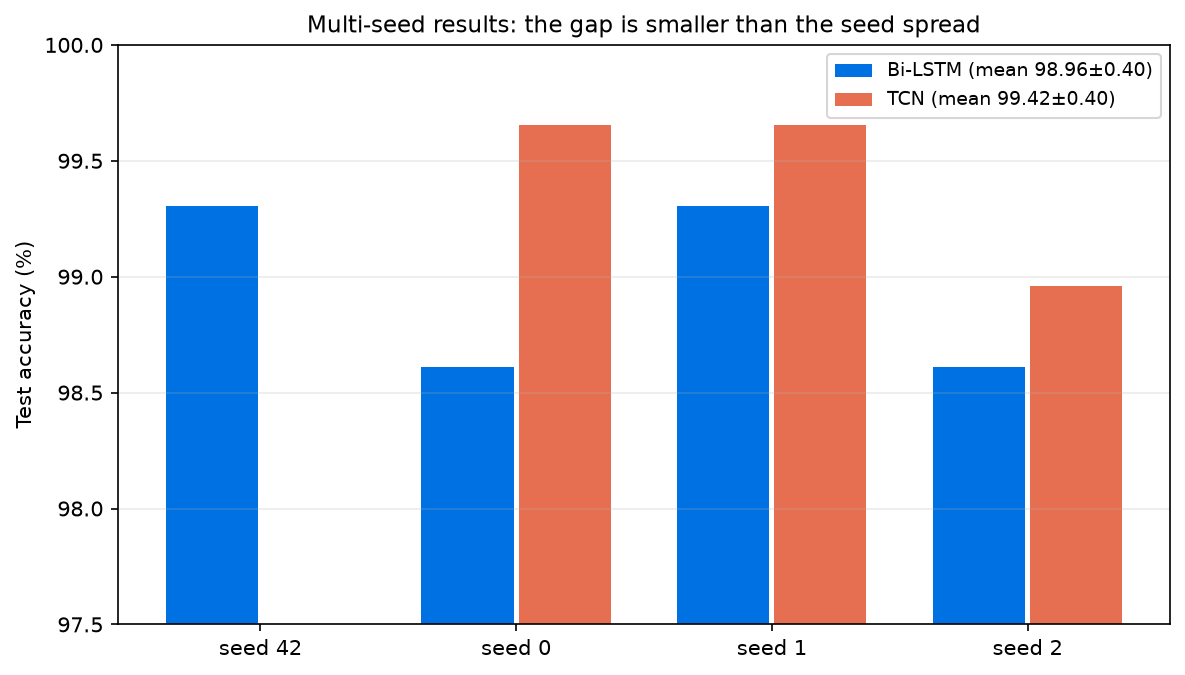
\includegraphics[width=0.85\textwidth]{fig5_multiseed.png}
\caption{Multi-seed test accuracy. The between-architecture gap (0.46\,pp) is smaller than the seed standard deviation (0.40\,pp); TCN was not run at seed 42 on environment B.}
\label{fig:seeds}
\end{figure}

The mean difference between TCN and Bi-LSTM is 0.46\,pp, which is smaller than the seed standard deviation of 0.40\,pp: the two architectures are therefore indistinguishable on this dataset, and the appropriate description is that they are of comparable accuracy rather than an advantage for either. TCN also converged in 5--6 epochs against 34--37 for Bi-LSTM, and reached 100.00\% validation accuracy in all three seeds, so it delivers the same accuracy at roughly 1/50 of the parameter count (0.30\,M vs 16.15\,M).

The training curve of the representative run (Figure~\ref{fig:curves}) falls monotonically from a loss of 3.08 to about 0.019 with training accuracy 99.61\%, while validation accuracy tracks it and plateaus; there is no evidence of overfitting at the reference setting. The confusion matrix (Figure~\ref{fig:cm}) shows four errors out of 288, all of which fall in class pairs that a pre-training similarity analysis had already flagged as most confusable (e.g.\ Television$\rightarrow$Like, $r=0.857$).

\begin{figure}[htbp]\centering
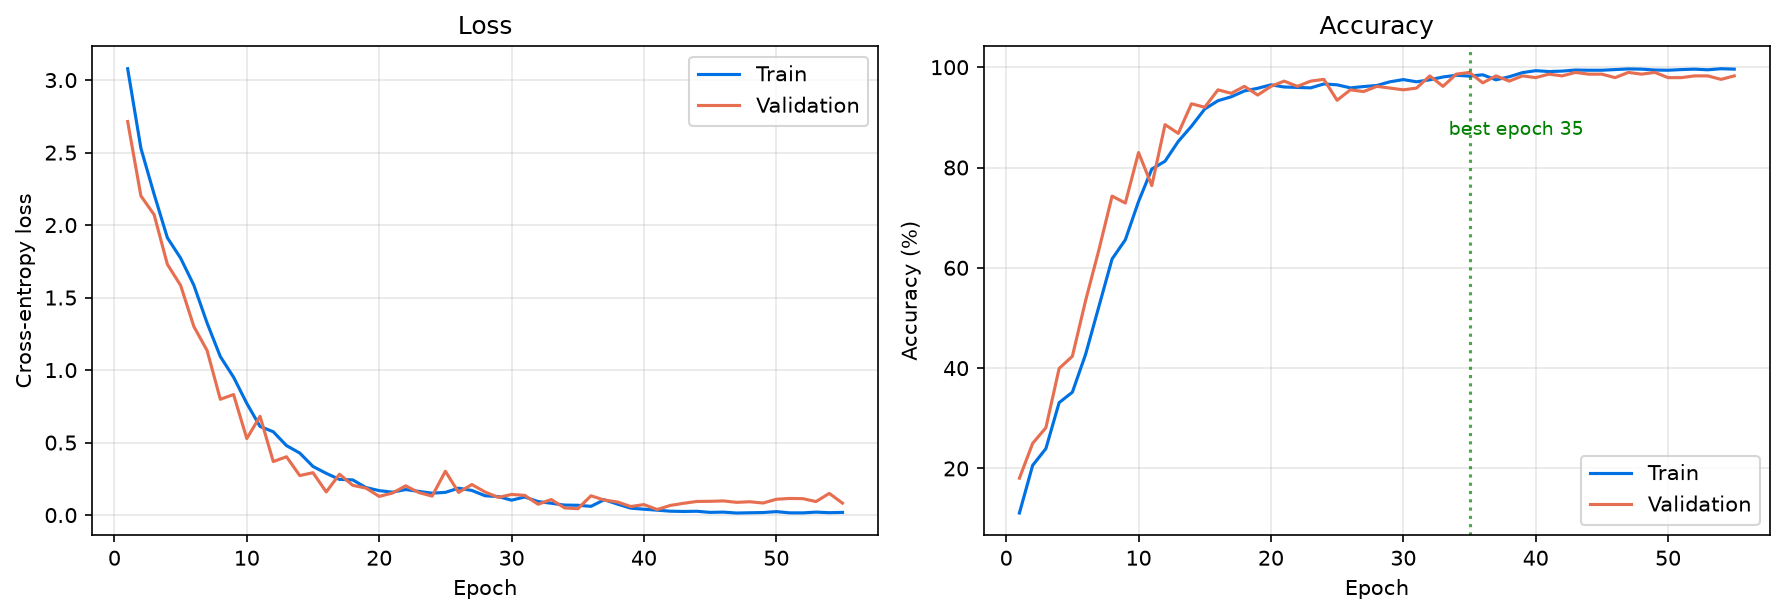
\includegraphics[width=0.92\textwidth]{fig2_curves.png}
\caption{Loss and accuracy during training of the representative fusion run (environment A, seed 42). The best validation accuracy is reached at epoch 35.}
\label{fig:curves}
\end{figure}

\begin{figure}[htbp]\centering
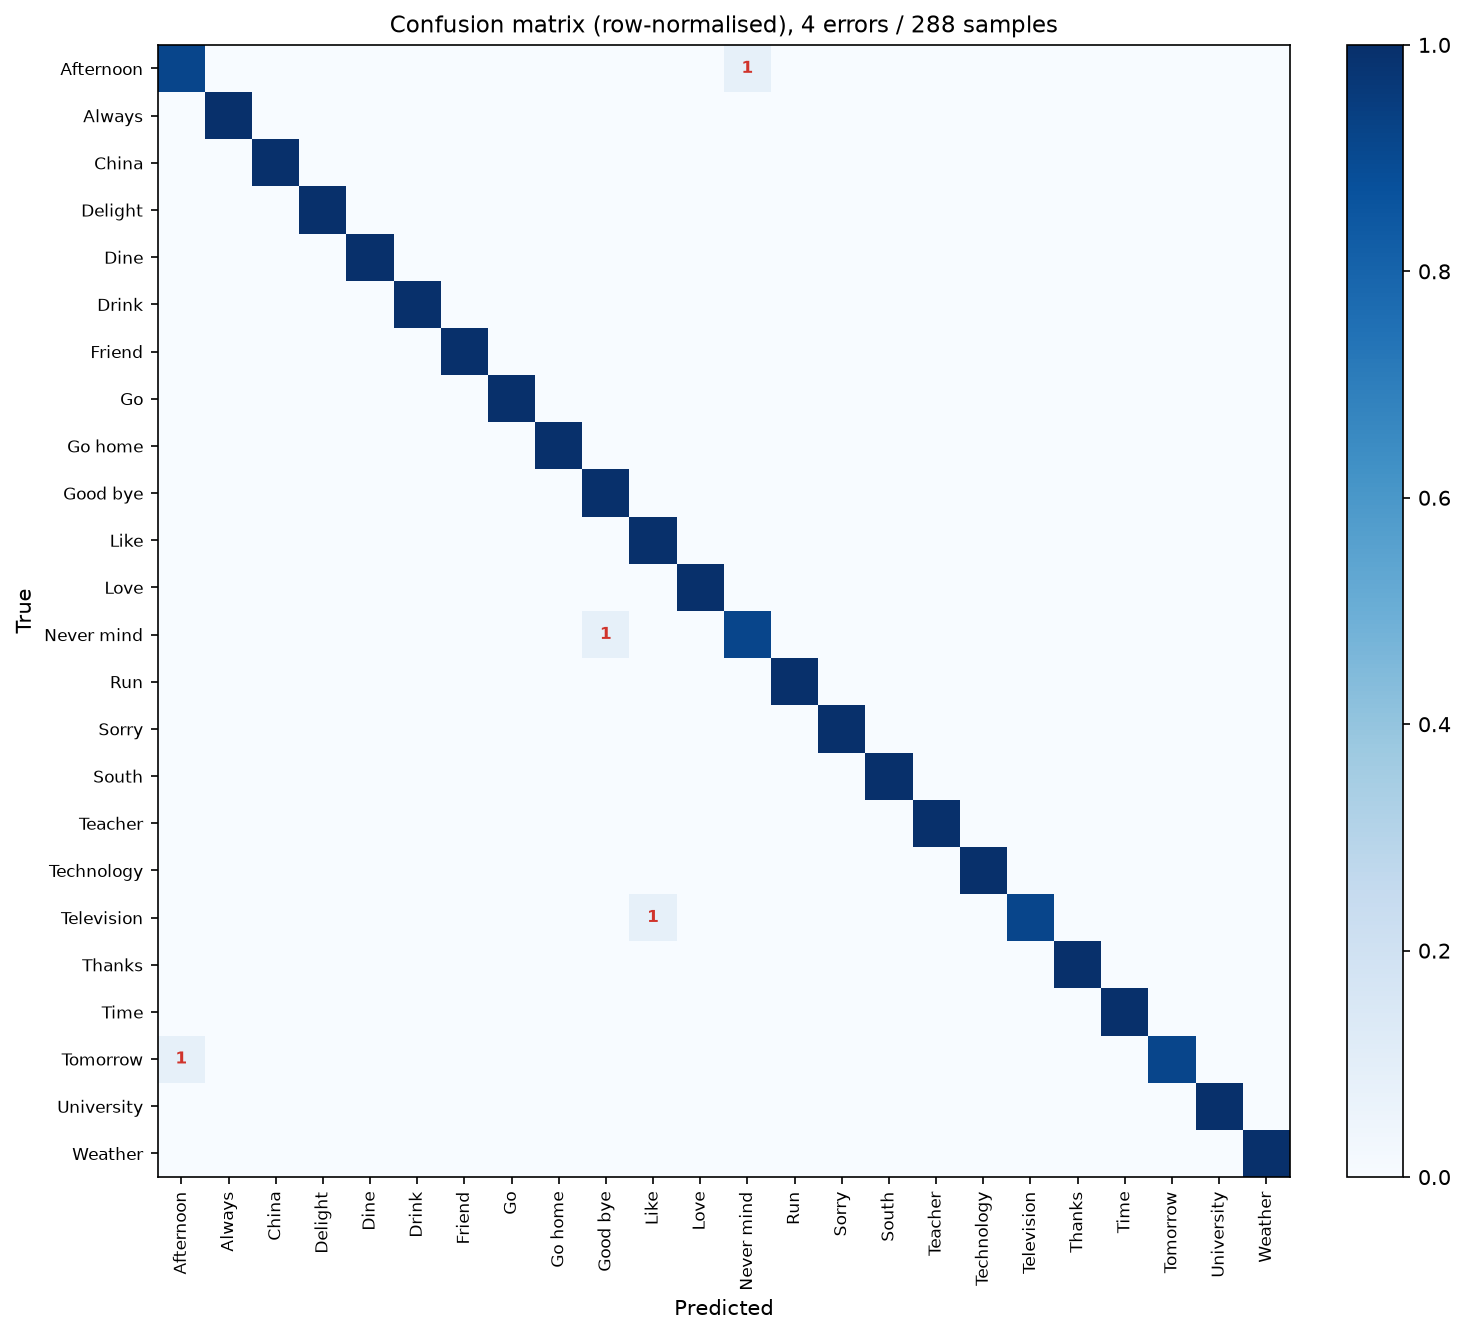
\includegraphics[width=0.78\textwidth]{fig3_confusion.png}
\caption{Confusion matrix of the fusion model on the 288-sample test set (row-normalised). Only four samples are misclassified.}
\label{fig:cm}
\end{figure}

\subsection{Parameter tuning}
\label{sec:tuning}

We swept learning rate, batch size and dropout one at a time under a fixed 40-epoch budget, holding the other parameters at reference values (Table~\ref{tab:tuning}). Learning rate 0.005 destabilises training (validation drops to 96.53\%), dropout 0.5 over-regularises (validation 96.18\%), and batch size 32 is the most favourable value. Taken individually, the highest-accuracy settings in the sweep are learning rate 0.002, batch size 32 and dropout 0.1.

\begin{table}[htbp]\centering
\caption{One-at-a-time parameter sweep (40-epoch budget, fusion input).}
\label{tab:tuning}
\begin{tabular}{lccc}
\toprule
Parameter & Value & Validation (\%) & Test (\%) \\
\midrule
\multirow{4}{*}{Learning rate} & 0.0005 & 98.26 & 97.92 \\
 & 0.001 & 98.61 & 98.61 \\
 & 0.002 & 98.61 & \textbf{98.96} \\
 & 0.005 & 96.53 & 98.61 \\
\midrule
\multirow{3}{*}{Batch size} & 16 & 98.96 & 98.61 \\
 & 32 & 99.65 & \textbf{99.31} \\
 & 50 & 98.61 & 98.61 \\
\midrule
\multirow{3}{*}{Dropout} & 0.1 & 99.31 & \textbf{99.31} \\
 & 0.3 & 98.61 & 98.61 \\
 & 0.5 & 96.18 & 97.57 \\
\bottomrule
\end{tabular}
\end{table}

However, combining the three individually highest-accuracy values does not preserve their benefit (Table~\ref{tab:combo}). The combination reaches only 98.26\%, below every individual setting, because it overfits: the final-epoch training accuracy is 100.00\% while validation accuracy stalls at 96.88\%. Low dropout (0.1) combined with a higher learning rate (0.002) lets the model memorise the training split faster than it can generalise. We therefore adopt learning rate $10^{-3}$, batch size 32 and dropout 0.3 --- that is, the reference setting with only the batch size changed --- which reaches 99.31\% and is the best Bi-LSTM result in this study.

\begin{table}[htbp]\centering
\caption{Combination check. Individually optimal hyperparameters do not compose.}
\label{tab:combo}
\begin{tabular}{lcccc}
\toprule
Configuration & LR & Batch & Dropout & Test (\%) \\
\midrule
Reference & $10^{-3}$ & 50 & 0.3 & 98.61 \\
Best batch size & $10^{-3}$ & 32 & 0.3 & \textbf{99.31} \\
Best learning rate & $2\times10^{-3}$ & 50 & 0.3 & 98.96 \\
Best dropout & $10^{-3}$ & 50 & 0.1 & 99.31 \\
Combination of all three & $2\times10^{-3}$ & 32 & 0.1 & 98.26 \\
\bottomrule
\end{tabular}
\end{table}

\subsection{Ablation study}

Removing individual components from the fusion model degrades accuracy in every case except one, which we treat separately (Table~\ref{tab:ablation}). Removing the two fully connected layers from each branch costs 2.43\,pp, reducing the temporal stack from three layers to one costs 3.82\,pp, and replacing concatenation with element-wise summation costs 1.04\,pp. The bidirectional property is the exception: the unidirectional variant reaches only 58.68\% and, importantly, its \emph{training} accuracy also stalls at 57\%. This is underfitting rather than a loss of generalisation, and we therefore do not interpret it as evidence that bidirectionality is required; we record it as an optimisation difficulty of single-direction LSTMs on 1,950-step sequences.

\begin{table}[htbp]\centering
\caption{Ablation of the fusion model (60-epoch budget).}
\label{tab:ablation}
\begin{tabular}{lccc}
\toprule
Variant & Test (\%) & $\Delta$ (pp) & Parameters (M) \\
\midrule
A0 Full model & \textbf{98.96} & --- & 16.15 \\
A1 Remove branch FC layers & 96.53 & $-2.43$ & 15.78 \\
A2 Bidirectional $\rightarrow$ unidirectional & 58.68 & $-40.28$ & 5.88 \\
A3 Three layers $\rightarrow$ one layer & 95.14 & $-3.82$ & 2.76 \\
A4 Concatenation $\rightarrow$ summation & 97.92 & $-1.04$ & 16.15 \\
\bottomrule
\end{tabular}
\end{table}

\subsection{Modality comparison}

Training three input configurations with otherwise identical settings gives fusion 98.61\%, glove-only 98.26\% and sEMG-only 91.32\% (Table~\ref{tab:modality}). The ordering agrees with the reference paper, but the fusion benefit is only $+0.35$\,pp here against the $+15.9$\,pp reported there, while glove-only accuracy is 14.5\,pp higher than reported.

\begin{table}[htbp]\centering
\caption{Single-modality versus fused input.}
\label{tab:modality}
\begin{tabular}{lccc}
\toprule
Input & Test (\%) & This work & Source paper \\
\midrule
Glove (strain/pressure) only & 98.26 & & 83.75 \\
sEMG only & 91.32 & & 88.02 \\
Fused & \textbf{98.61} & & 99.65 \\
\bottomrule
\end{tabular}
\end{table}

\begin{figure}[htbp]\centering
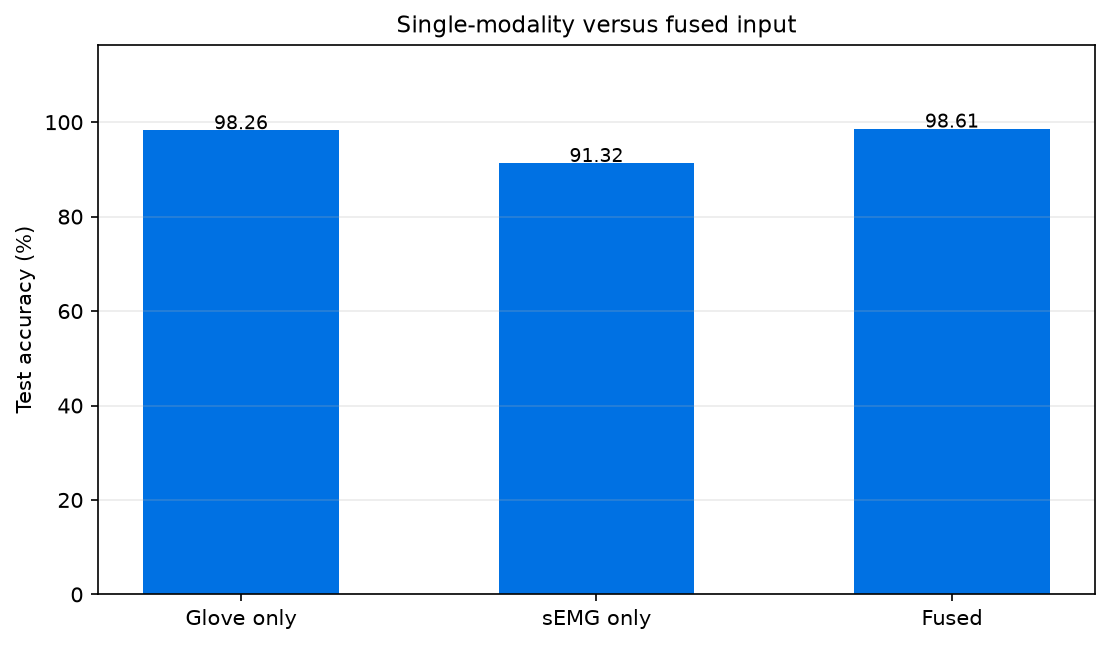
\includegraphics[width=0.7\textwidth]{fig4_modality.png}
\caption{Test accuracy for single-modality and fused inputs. The fusion benefit over glove-only input is 0.35\,pp, far below the $+15.9$\,pp reported by the reference system.}
\label{fig:modality}
\end{figure}

\subsection{Modality dependence: inference pruning}
\label{sec:prune}

Comparing separately-trained single-modality models does not reveal what a \emph{fused} model actually uses at inference. We test this directly by loading the trained fusion model and zeroing one input branch while keeping the weights fixed (Table~\ref{tab:prune}).

\begin{table}[htbp]\centering
\caption{Inference pruning on the fitted fusion model (288 test samples).}
\label{tab:prune}
\begin{tabular}{lccc}
\toprule
Checkpoint & Full fusion (\%) & Glove only (\%) & Identical predictions \\
\midrule
Baseline (seed 42) & 99.31 & 99.31 & \textbf{288/288} \\
Modality dropout 30\% & 98.96 & 98.96 & \textbf{288/288} \\
Modality dropout 50\% & 98.61 & 98.61 & \textbf{288/288} \\
\bottomrule
\end{tabular}
\end{table}

Zeroing sEMG leaves \emph{all} 288 predictions unchanged --- not merely the same error count, but identical labels sample by sample. Zeroing the glove input instead collapses accuracy to 4.17\%, which is exactly chance for 24 classes, and the model emits a single constant class for every input. The fitted "multimodal fusion" model is therefore functionally equivalent to a glove-only classifier, and the sEMG branch contributes exactly zero to the decision.

\subsection{Fusion mechanism experiments}
\label{sec:mech}

\textbf{Modality dropout.} If the model ignores sEMG because training did not force it to be useful, then randomly zeroing one branch during training should help. It does not. With dropout probability 0.5 --- so that 25\% of samples have the glove input zeroed and must be classified from sEMG alone --- the resulting model still ignores sEMG at inference (288/288 identical predictions after pruning) and its accuracy is slightly lower (98.61\% vs 99.31\%).

The training dynamics explain why. That model's final training accuracy is 0.7617, which matches the value expected if the 75\% of samples with both modalities visible are classified correctly and the 25\% with a zeroed glove input are not: $0.75\times100\% + 0.25\times4\% \approx 0.76$. The optimiser therefore sacrifices a quarter of the training set rather than learn the sEMG branch --- the branch is not merely under-trained, it is not learnable through this optimisation path at this data scale.

\textbf{sEMG filtering.} Section~\ref{sec:methods} noted that 45.9\% of sEMG energy lies in 1--20\,Hz drift and 18.7\% in a narrow 48.17\,Hz interference line, with only 11.2\% in the 51--450\,Hz band normally associated with muscle activity. The intuitive remedy is to filter, and we tested it with a 4th-order Butterworth band-pass (20--450\,Hz) plus notches at 48.17\,Hz and its harmonics. Filtering does remove the unwanted energy (1--20\,Hz falls to 2.5\%, the 48\,Hz line to 0.4\%), but it reduces single-modality accuracy from 89.24\% to 75.69\%, a loss of 13.55\,pp (Table~\ref{tab:filter}). The low-frequency content we assumed to be noise is in fact discriminative.

Filtering does, however, change the fusion dynamics in an informative way. The filtered-fusion model \emph{does} use sEMG: pruning it to the glove branch drops accuracy by 36.46\,pp (from 95.49\% to 59.03\%), against 0.00\,pp for the unfiltered model. In other words, filtering makes the sEMG features exploitable by the classifier head, but at the cost of removing information, so the modality becomes simultaneously usable and weaker, and overall accuracy falls.

\begin{table}[htbp]\centering
\caption{sEMG filtering: comparison and pruning behaviour.}
\label{tab:filter}
\begin{tabular}{lcccc}
\toprule
Configuration & Unfiltered (\%) & Filtered (\%) & $\Delta$ (pp) & Pruning to glove (pp) \\
\midrule
sEMG only & \textbf{89.24} & 75.69 & $-13.55$ & --- \\
Fused & \textbf{99.31} & 95.49 & $-3.82$ & $+0.00$ / $\mathbf{-36.46}$ \\
\bottomrule
\end{tabular}
\end{table}

\textbf{Oracle upper bound.} Finally we ask whether any fusion strategy could have helped. For each test sample we mark a hit if \emph{either} the glove model or the sEMG model predicts correctly; this bound is unreachable by any real fusion rule and therefore upper-bounds what improved training could achieve (Table~\ref{tab:oracle}).

\begin{table}[htbp]\centering
\caption{Oracle upper bound. In four of five configurations the bound equals the observed score, leaving no reachable improvement.}
\label{tab:oracle}
\small
\setlength{\tabcolsep}{4.5pt}
\begin{tabular}{lccccc}
\toprule
Model / environment & Observed & sEMG-only & Oracle & Headroom (pp) & Both wrong \\
\midrule
Bi-LSTM, environment A & 98.61 & 91.32 & 98.96 & $+0.35$ & 3 \\
TCN, environment A & 99.65 & 91.32 & \textbf{99.65} & $\mathbf{+0.00}$ & 1 \\
1D-CNN, environment A & 99.31 & 91.32 & \textbf{99.31} & $\mathbf{+0.00}$ & 2 \\
Bi-LSTM, environment B & 99.31 & 89.24 & \textbf{99.31} & $\mathbf{+0.00}$ & 2 \\
TCN, environment B & 99.65 & 89.24 & \textbf{99.65} & $\mathbf{+0.00}$ & 1 \\
\bottomrule
\end{tabular}
\end{table}

In four of five configurations the oracle bound is identical to the observed accuracy: no correction to the fusion mechanism can improve the result. The single exception has 1 sample (0.35\,pp) of headroom, below the 0.40\,pp seed standard deviation. Examining where the baseline errs is equally informative: its two errors on environment B are also wrong for the sEMG model, while 29 samples (10.1\%) that the baseline classifies correctly are wrong for sEMG --- so involving sEMG would risk losing accuracy rather than gaining it.

%=====================================================================
\begin{figure}[htbp]\centering
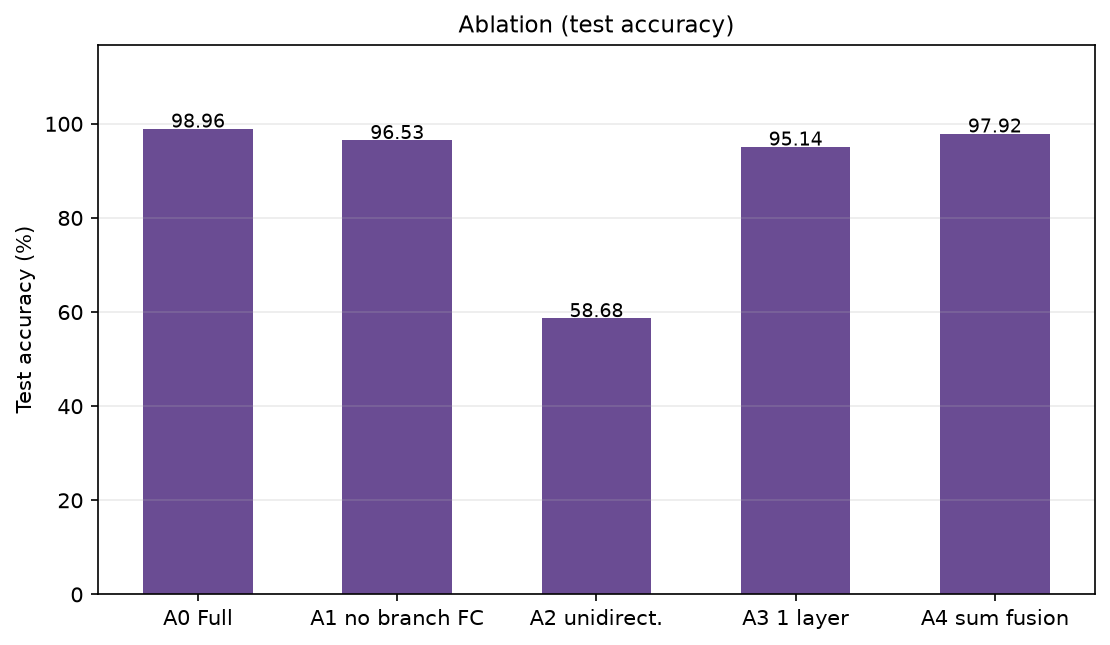
\includegraphics[width=0.8\textwidth]{fig6_ablation.png}
\caption{Ablation results. All variants except A2 lose accuracy relative to the full model; A2's loss reflects underfitting (its training accuracy stalls at 57\%) rather than reduced generalisation.}
\label{fig:ablation}
\end{figure}

\section{Discussion}

\textbf{Why the fusion gain does not reproduce.} The reference paper reports that fusion exceeds glove-only accuracy by 15.9\,pp; we observe 0.35\,pp, and the pruning experiment shows the fused model does not use its sEMG input at all. The two observations are consistent once the glove channel's standalone accuracy is considered: in this dataset glove-only reaches 98.26\% (environment A) to 99.31\% (environment B). A classifier that already separates nearly every sample through one branch receives no gradient signal encouraging it to exploit the other, so the second branch is effectively pruned by the optimiser itself. This is the dominant-modality regime, and it predicts precisely what we measure: an oracle bound equal to the observed score, and an sEMG branch whose removal is invisible.

The divergence from the reference therefore does not concern the fusion mechanism, which we implemented to specification, but the difficulty of the glove-only problem. If the reference system's glove-only accuracy were 83.75\%, fusion would have real headroom there. We cannot resolve which factor produces that difference: the reference paper's supplementary material describing the single-modality protocol was not available to us, and the candidates --- a different evaluation protocol, a different model for the single-modality comparison, or a different data version --- are not separable from the published information. We state this as an open question rather than attributing it.

\textbf{Why filtering backfires, and what it reveals.} The low-frequency energy in sEMG is usually attributed to baseline drift and treated as noise. Our filtering experiment contradicts this: removing 43\,pp of low-frequency energy costs 13.55\,pp of accuracy. A plausible reading is that the 1--20\,Hz content carries the envelope of the gesture dynamics, which correlates with class membership under a fixed electrode placement. The same experiment also shows that the sEMG branch is not intrinsically unusable --- once the features are cleaner, the classifier head does integrate them (pruning cost 36.46\,pp) --- but the underlying signal has by then lost information, so the net effect is negative. This separates two questions that accuracy alone conflates: whether a branch \emph{can} be used, and whether using it \emph{helps}.

\textbf{Implications for multimodal wearable sensing.} Our results caution against reading a large fusion gain as a property of the modality pair. The gain depends on the headroom left by the strongest single channel: with a near-ceiling modality, added sensors contribute nothing measurable even when the fusion architecture is correct. This suggests that claims of multimodal benefit should be accompanied by the single-modality baseline on the same split --- which we provide here --- and by an upper bound such as the oracle analysis, which costs no training and directly states how much is at stake.

\textbf{Reproducibility observations.} Two effects are worth recording because they are usually invisible. First, identical code, data, seed and library versions produced different training trajectories on two GPUs, differing by 0.70\,pp in final accuracy; the cause is algorithm selection inside cuDNN rather than any error in the pipeline. Second, near-duplicate samples across a random split inflated accuracy by 0.52\,pp, a property of repeated-trial acquisition that a random split cannot avoid.

%=====================================================================
\section{Conclusion}

We reproduced a multimodal Chinese Sign Language recognition system on its own 24-class dataset and matched its reported fused accuracy within random-seed variance: 98.61\% in a single run and $98.96\pm0.40$\% over four seeds, with TCN comparators at $99.42\pm0.40$\% and the split verified byte-identical across two environments (\textbf{C1}). We then showed, through three mutually independent experiments, that the fused model is functionally unimodal: inference pruning leaves all 288 predictions unchanged when sEMG is zeroed, modality dropout cannot force the branch to be used, and an oracle bound equals the observed accuracy in four of five configurations, leaving no reachable improvement (\textbf{C2}). Finally, we quantified the seed variance (0.40\,pp), the near-duplicate inflation ($+0.52$\,pp), the cross-GPU trajectory divergence at fixed seed, and falsified the low-frequency-noise filtering hypothesis at a cost of 13.55\,pp (\textbf{C3}). The practical reading is that, on this dataset, the fusion architecture is not the limiting factor --- the glove modality alone already solves the task, and no fusion strategy has room to contribute.

%=====================================================================
\section{Limitations and Future Work}

\textbf{Statistical resolution.} The test set contains 288 samples, so single-run differences below about 1\,pp are not resolvable. We mitigate this with four seeds on the primary model, but several secondary comparisons rest on single runs and should be read as indicative.

\textbf{Near-duplicate inflation.} 27.4\% of test samples have a near-identical training neighbour, inflating fused accuracy by 0.52\,pp. A group-aware split that assigns near-duplicates to the same side would isolate the duplicate-free accuracy; we report the stratified estimate instead so as to preserve the reference random-split protocol.

\textbf{Unresolved divergence from the reference.} The single-modality protocol used by the reference system could not be verified, so the 14.5\,pp gap in glove-only accuracy remains unexplained. Direct comparison would require either their supplementary material or their evaluation code.

\textbf{Remedies not attempted.} Given the oracle bound, training-side interventions aimed at the fusion mechanism --- gradient balancing, per-branch auxiliary supervision, attention-based fusion --- have no reachable benefit on this dataset, and we did not implement them. They would become relevant on a dataset where the dominant modality leaves measurable headroom.

\textbf{Cross-environment reproducibility.} Trajectories diverge between GPU models at fixed seed. Exact bitwise reproduction across heterogeneous hardware would require deterministic kernel selection, which typically costs throughput; we instead control for it by comparing only within one environment.

%=====================================================================
\begin{thebibliography}{9}
\small
\bibitem{ref1} The reference multimodal sign-language recognition system studied here (source system report, 2026). Its supplementary material, which describes the single-modality evaluation protocol, was not available at the time of writing.

\bibitem{ref2} Hochreiter, S., Schmidhuber, J. Long short-term memory. \emph{Neural Computation} 9(8), 1735--1780 (1997).

\bibitem{ref3} Loshchilov, I., Hutter, F. Decoupled weight decay regularization. \emph{ICLR} (2019).

\bibitem{ref4} Bai, S., Kolter, J. Z., Koltun, V. An empirical evaluation of generic convolutional and recurrent networks for sequence modeling. arXiv:1803.01271 (2018).

\bibitem{ref5} Chen, Z., Badrinarayanan, V., Lee, C.-Y., Rabinovich, A. GradNorm: Gradient normalization for adaptive loss balancing in deep multitask networks. \emph{ICML} (2018).

\bibitem{ref6} Yu, T., Kumar, S., Gupta, A., Levine, S., Hausman, K., Finn, C. Gradient surgery for multi-task learning. \emph{NeurIPS} (2020).

\bibitem{ref7} Wang, W., Tran, D., Feiszli, M. What makes training multi-modal classification networks hard? \emph{CVPR} (2020).
\end{thebibliography}

\appendix
\section{Appendix: Full run inventory and per-class results}

\begin{table}[htbp]\centering
\caption{A1. All trained configurations reported in this work. ``Environment'' distinguishes the two GPU environments of Section~\ref{sec:env}; only same-environment comparisons are drawn in the main text.}
\label{tab:inventory}
\footnotesize
\setlength{\tabcolsep}{4pt}
\begin{tabular}{llcccl}
\toprule
Tag & Configuration & Host & Epochs & Test (\%) & Section \\
\midrule
\texttt{bilstm\_both} & Fusion, epoch budget 100 & A & 55 & 98.61 & \ref{sec:main} \\
\texttt{remote\_verify} & Fusion, epoch budget 100 & B & 49 & 99.31 & \ref{sec:env} \\
\texttt{p3\_bilstm\_s0/1/2} & Fusion, seeds 0/1/2 & B & 60 & 98.61 / 99.31 / 98.61 & \ref{sec:main} \\
\texttt{p3\_tcn\_s0/1/2} & TCN, seeds 0/1/2 & B & 60 & 99.65 / 99.65 / 98.96 & \ref{sec:main} \\
\texttt{modality\_glove} & Glove only & A & 60 & 98.26 & \ref{sec:results} \\
\texttt{modality\_semg} & sEMG only & A & 60 & 91.32 & \ref{sec:results} \\
\texttt{p2\_base\_semg} & sEMG only & B & 60 & 89.24 & \ref{sec:mech} \\
\texttt{p2\_filter\_semg} & sEMG only, filtered & B & 60 & 75.69 & \ref{sec:mech} \\
\texttt{p2\_filter\_both} & Fusion, filtered & B & 60 & 95.49 & \ref{sec:mech} \\
\texttt{p1\_moddrop30/50} & Modality dropout 30\% / 50\% & B & 60 & 98.96 / 98.61 & \ref{sec:mech} \\
\texttt{best\_combo} & LR 0.002, batch 32, dropout 0.1 & A & 40 & 98.26 & \ref{sec:tuning} \\
\bottomrule
\end{tabular}
\end{table}

\begin{table}[htbp]\centering
\caption{A2. Per-class recall of the representative fusion run, ascending. Classes below 1.0 share handshape or motion similarity with a neighbouring class.}
\label{tab:perclass}
\small
\begin{tabular}{lcc}
\toprule
Class & Test samples & Recall (\%) \\
\midrule
Afternoon & 12 & 91.7 \\
Never mind & 12 & 91.7 \\
Tomorrow & 12 & 91.7 \\
Television & 12 & 91.7 \\
Other 20 classes & 240 & 100.0 \\
\bottomrule
\end{tabular}
\end{table}

\noindent\textbf{Complete error list (representative run).} Television$\rightarrow$Like (1; class-pair Pearson $r=0.857$), Tomorrow$\rightarrow$Afternoon (1), Never mind$\rightarrow$Good bye (1), Afternoon$\rightarrow$Never mind (1).

\end{document}
